% Chapter 4

\chapter{Automated Software Release} % Main chapter title 
\label{Chapter 4}

In Chapter \ref{Chapter2}, some of the basic concepts and terminologies involved in the software development and release process were discussed. In continuation, this chapter outlined the ongoing process of software release (see Section~\ref{section:OngoingProcessofSoftware Release}) within the department and highlight few shortcomings (see Section~\ref{section:Opportunities for Improvement}). Furthermore, based on the versioning utility tools (see Section~\ref{section:Standard-Version}), the analysis and the implementation concept of an automated software release is discussed, considering an example software component (see Section~\ref{section:implementationconcept}). With the solution approach, this chapter intends to answer the following question.




\vspace{0.2cm}
\noindent Question 2: How to automate the software release process in respect to version control ?


%----------------------------------------------------------------------------------------


\section{Ongoing Process}\label{section:OngoingProcessofSoftware Release}

To increase the understanding of the software release lifecycle, it is imperative to know the enterprise strategy and goals behind a software release and understand its implications. Since, the release cycle is significantly vast with multiple steps in an incremental software development process, this section gives more focus on the area of the version release control for a specific software package. The customer project follows an agile development model where the actual development work is divided into smaller iterative tasks defined over a dedicated period known as sprints. Incremental development of the software project is executed with the goal of delivering an optimal subset of requirements in a certain release~\parencite{wohlin2005important}. The ongoing release process also follows the typical approach highlighted in Section~\ref{section:Softwareconfigurationmanagement} under title "Release Management". At the end of each release cycle, a new version of the software product or the project gets introduced. It is either intended for external customers or internal deployment purpose. An increment or an introduction of the version number after a successful release follows the same terminology mentioned in the "Software versioning" part under Section~\ref{section:Softwareconfigurationmanagement}. This is done with the help of git tags if the project is hosted over the GitHub platform. Tags capture a particular point of the project which can be released and is independent of branches. It holds the new features and modifications to the existing codebase. A key importance of release versioning is that anyone can refer to the history of commits and track changes committed to a project and this potentially improves the quality of the codebase and its maintainability. 


But, there is a challenge involved in the present release cycle for the development projects within the department. The process needs manual intervention of the developers for bumping or increasing the software version number upon the end of each release and it is a little inefficient work, given its description.



%----------------------------------------------------------------------------------------
\section{Area of Improvement}\label{section:Opportunities for Improvement}

To quantify the importance of release versioning, the developers needs to understand few key things that are maintained in the release process and consider various ways for improvements, if shortcomings are found. As mentioned in the preceding section, the struggle to manually update versions and create git tags is substantial. Above this, the developer also must generate a changelog file manually, to record all the changes based on the commit messages. A \emph{Changelog} is a file used within the project repository to document all the changes for each version and is usually named "CHANGELOG.md". 

To avoid the manual hassle mentioned aforesaid, the thesis explores solution to automate the process of versioning. While there are many potential tools that can fulfil the requirement of automating software release, this research presents a powerful "standard-version" utility tool and studies its effectiveness. With standard-version, versioning can be easily automated as well as changelog generation and modification can be handled automatically. It is based on conventional commit messages and semantic versioning concept, where each change or an increment of the version number denotes a certain meaning. \emph{Semantic Versioning} or \ac{SemVer} is a common set of versioning practice well recognised by the software developers that explains how version numbers are defined or incremented. In addition to the versioning terminologies mentioned previously, a small change or bug fix that does not break the \ac{API} increments the patch number, backward compatible \ac{API} changes or additions increments the minor number, resetting the last number to zero and the major number is incremented when backward incompatible changes or additions are introduced, setting the other numbers to zero~\parencite{preston2013semantic}.

\section{Conventional Commits} 

The Conventional Commits is a way to structure commit messages to a project repository based on the concept of semantic versioning. It offers to generate conventional changelog out of the conventional commit messages and utility tools like the standard version can work on top of it. Refer to following listing ~\ref{lst:listing-conventionalcommits} to learn more about the structure of the conventional commits message. Here, a commit type "fix" represents a bug fix and correspond to the patch number in \ac{SemVer} and a a commit type "feat" represents any additional feature introduced to the software and the same correspond to the minor version number. However, a footer message with "BREAKING CHANGE" or a type/scope followed by a "!" corresponds to the major version number and denotes a breaking API change. Developers can also add other types like "docs" or "build", but it does not have any direct effect on the version numbers. 

\vspace{0.5cm}
\lstset{style=mystyle}
\lstinputlisting[caption= An example structure of the conventional commit message, captionpos=b, basicstyle=\footnotesize, stepnumber=1, frame=lines, numbers=left, label={lst:listing-conventionalcommits}, language=python]{code/conventionalcommits}
\vspace{0.5cm}

As highlighted above, the feature is standardized across various software projects and is welcomed by the developers\footnote{Refer to the official conventional commits specification document for more details}. It has also been introduced in one of the project within the department as a part of this research. In the later sections, the thesis also analyses the impact of conventional commits on the automated versioning tools such as the standard-version. Besides, a pre-commit hook can also be installed on the local git repository to verify the commit messages prior to the actual commit and push.  

%~\parencite{ConvComm}

\section{Standard Version Utility}\label{section:Standard-Version}

With standard-version utility, the task of software release becomes simple. It collaborate well with conventional ecosystem and \ac{SemVer}. If used locally, the utility handles the job of version bump in accordance with the last conventional commit messages without automatically pushing to the GitHub remote repository. Depending on the intended use case, standard-version gives the opportunity to review the release state from the local repository itself before publishing a new git tag or the updated version number to the remote resource. It can generate a pre-release and allow customization of the git tag format, changelog generation and also add commit types (feat and fix are default types). To comprehend the functionality of this tool, refer to figure \ref{fig:Standard-Version} where the automated release process is highlighted involving multiple git branches. Here, changes to the codebase are committed using the conventional commit types and then pushed to the feature branch A and B and then merged into the main or the master branch. After a successful merge, the standard-version command will take charge of the automated release and fulfil the following jobs. 

\begin{itemize}

\item Retrieve the last version number of the software component\footnote{Achieved by identifying the latest git tag in a certain project repository}
\item Increment the version number based on the conventional commit types
\item Additionally, update the version in an user-defined file as well where the version should be incremented
\item Generate or update the project changelog
\item Create a new git tag with the updated version number

\end{itemize}


\vspace{0.5cm}
\begin{figure}[H]
\begin{tikzpicture}[node distance=2.0cm, inner sep=2mm, minimum width=1.5cm, >=stealth']
\node [draw, rectangle, drop shadow, fill=gray!30] (V) at (0,0) {Feature branch A};
\node [right=of V] (mech) at (3,0) {commit -m "feat(scope): description"};
\node [right=of C] (standard) at (8,-3) {version bump};
\node [draw, circle, drop shadow, fill=gray!30, text width=2cm, align=center] (C) [below right=of V] {Master branch};
\node [draw, rectangle, drop shadow, fill=gray!30] (D) [below right=of C] {Feature branch B};
\node [left=of D] (mechB) {commit -m "fix(scope): description"};

\node (ctrl1) [above=of D] {};
\node (ctrl3) [right=of C] {};
\node (ctrl4) [above right=of D] {};

\path [draw, ->, dashed] (V) edge node [fill=white] {merge} (C);
\path [draw, ->, dashed] (mech) edge node [fill=white] {push} (V);
\path [draw, ->, dashed] (mechB) edge node [fill=white] {push} (D);
\path [draw, ->, dashed] (C) edge node [fill=white] {standard-version} (standard);
\path [draw, ->, dashed] (standard) edge [bend right] node [fill=white] {push - -follow-tags} (C);
\path [draw, ->, dashed] (D) edge node [fill=white] {merge} (C);
\end{tikzpicture}
\vspace{0.2cm}
\caption[Control flow graph to automate the software release using standard-version utility]{Control flow graph of automated software release and version bump using the standard-version utility. Here, the scope and description of the commit message can be specified according to the committed changes}
\label{fig:Standard-Version}
\end{figure}
\vspace{0.5cm}


After successfully reviewing the release state, the updated version number and the git tag is pushed back to the master branch. The thesis makes further progress by leveraging the existing functionality offered by the standard-version utility, and configure a pipeline job as a part of the \ac{CI} \ac{CD} to supervise the software release process with continuous release.

\section{Implementation Approach}\label{section:implementationconcept}

The project repositories are configured in such a way that it allows easy building of software packages and provide cross-compilation support as the intended packages are meant to be built on a different platform and not the one where it is compiled for initial development. Thereby, configuration files like "CMakeLists.txt" are implemented in the root directory of the project codebase with all the necessary user-defined files. These configuration files are required to generate the build files, which ultimately helps the software for cross-platform development. Consequently, one necessary file is the version text file amongst others, specified for the "CMakeLists.txt" to store the current project version. The build system reads this version number from the text file during the software build. Depending on the use case and the project complexity, the configuration to store the current project version can be handled in various ways. In regards to this project implementation, the current version of the software is set with the "version.txt" file and is kept independent of the release tags on the GitHub platform.

With each development release, the version number is updated in the text file and a new tag is generated. The work experiments with one particular software component that is implemented within the department and tries to automate the software release process. The manual effort to update the version file and the creation of a new git tag with each release is reduced owing to the standard-version utility tool. Additionally, a Jenkins pipeline is configured to tackle the manual process and perform all the activities involved in the release of the software component. With new remote commits, the Jenkins build is executed which checks out the changeset\footnote{A changeset is defined as the collection of commits made on the codebase of a project repository} in the codebase and automatically increments the version number in the text file based on the committed message, creates a new tag and update the changelog. The following listing \ref{lst:listing-releasescript} demonstrates the release script implemented which handles the software release process. The git committer details are required to perform the standard-version command and determine the next version based on the commit message. 

\vspace{0.5cm}
\lstset{style=mystyle}
\lstinputlisting[caption= Implemented release script to manage the continuous release of an example software component, captionpos=b,basicstyle=\footnotesize, stepnumber=1, frame=lines, numbers=left, label={lst:listing-releasescript}, language=bash]{code/releasescript.sh}
\vspace{0.5cm}

Post release, the necessary changes to the version file, new git tag and the updated changelog are pushed back to the  
remote repository. As illustrated in Figure \ref{fig:Changelog}, the changelog will capture all the commits associated to the project codebase. At the first release, the standard-version utility will create a new changelog, if the same is missing.
\vspace{0.5cm}
\begin{figure}[H]
\centering{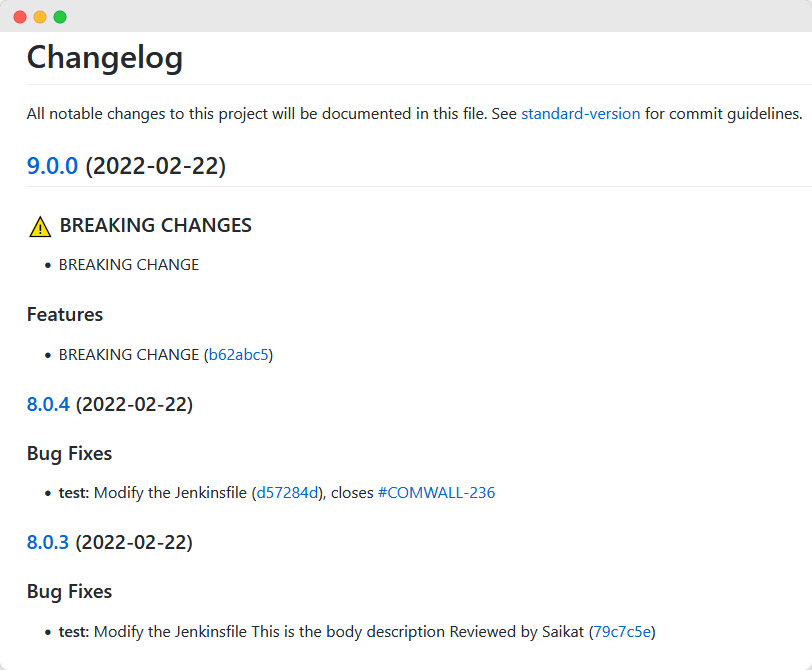
\includegraphics[width=1\textwidth]{figures/changelog.png} }%
\caption[The CHANGELOG.md file]{The CHANGELOG file to tracks changes related to each software version}
\label{fig:Changelog}
\end{figure}
\vspace{0.5cm}

















%----------------------------------------------------------------------------------------


\clearpage\null\thispagestyle{empty}